%%%%%%%%%%%%%%%%%%%%%%%%%%%%% CARATULA%%%%%%%%%%%%%%%%%%%%%%%%
\textheight 19cm
\pagestyle{empty}
\begin{center}
 {\bf {\fontsize{14}{16.8}\selectfont UNIVERSIDAD NACIONAL DE TRUJILLO}}     
 
    {\bf{\fontsize{14}{16.8}\selectfont Facultad de Ciencias Físicas y Matemáticas}} 

  {\bf{\fontsize{14}{16.8}\selectfont Escuela Profesional de Informática}}
\end{center}  

\begin{figure}[ht]
\begin{center}

\includegraphics[width=.4\textwidth]{Imagenes/Cap0/unt}
\end{center}
\end{figure}
\vskip 0.5cm

\begin{center}  
    {\bf\Large{{\fontsize{17}{20.4}\selectfont{} Sistema de seguridad para el control de acceso a una vivienda mediante el reconocimiento de voz utilizando coeficientes cepstrum MFCC Y DTW}}}
\end{center}   

\begin{center}
{\Large{TESIS}}
\end{center}
\begin{center}
{\large{\hspace*{0.4cm} PARA OPTAR EL TÍTULO PROFESIONAL DE INGENIERO  INFORMÁTICO}}
\end{center}

\vskip 0.6cm
\begin{center}
  { \fontsize{14}{16.8}\selectfont {\hspace{-2.9cm}AUTORES: Ocas Quiroz Carlos E.}} \\
    { \fontsize{14}{16.8}\selectfont {\hspace{-0.4cm} Sánchez Pedro Edwin J.}}\\
    \vskip 0.2cm
    { \fontsize{14}{16.8}\selectfont {\hspace{-1.7cm} ASESOR: Ms. Peralta Luján José L.}}
\end{center}  

\vskip 1.1cm
\begin{center}    
{\bf {\fontsize{14}{16.8}\selectfont TRUJILLO - PERÚ
\vskip 0.0cm
\hspace*{-0.2cm} 
2019 }}
\end{center} 
\newpage
%%%%%%%%%%%%%%%%%%%%%%%%%%%%%%%%%%%%%%%%%%%%%%%%%%%%%%%%%%%%%%%%%%%%%%%%%%%


%%%%%%%%%%%%%%%%%%%%%%%%%%%% DEDICATORIA %%%%%%%%%%%%%%%%%%%%%%
 \pagestyle{plain}
 \pagenumbering{roman}
 \addcontentsline{toc}{chapter}{Dedicatoria}
 {\bf\Large {Dedicamos esta tesis a :}}
 \vskip 1cm
\begin{quotation}
{\it Nuestras familias por el apoyo incondicional y permanente que nos brindaron durante nuestra preparación académica para poder llegar a ser profesionales competitivos y de éxito, quienes con su amor y paciencia permitieron cumplir un deseo tan esperado, y que ahora permite ser útil a nuestro país.}
\end{quotation}
%%%%%%%%%%%%%%%%%%%%%%%%%%%%%%%%%%%%%%%%%%%%%%%%%%%%%%%%%%%%%%%%%%%%%%%%%%%


%%%%%%%%%%%%%%%%%%%%%%%%%%%% AGRADECIMENTOS %%%%%%%%%%%%%%%%%%%%%%
\newpage

 \addcontentsline{toc}{chapter}{Agradecimientos}
 {\bf\Large {\flushleft{Agradecimientos}}}
\vskip 0.2cm
\begin{quotation}
A Dios y a nuestros padres, ya que sin ellos nada de esto hubiera sido posible.
{\vskip 0.2cm}
A nuestro asesor de tesis, Ms. José Peralta Luján, que, con su amistad, apoyo, paciencia, dedicación, consejos y observaciones en la realización de este trabajo pudimos sacar adelante esta tesis y además por darnos las herramientas necesarias para ser mejores profesionales cada día.
\vskip 0.2cm
Al Ing. Clayder Gonzales Cadenillas, que desde un principio se mostró siempre disponible e interesado, brindándonos su apoyo y motivándonos en esta área de investigación.
\vskip 0.2cm
A nuestros amigos, Ing. Javier Fuentes Huertas e Ing. Alexis Aspauza Lezcano, por el apoyo y consejos dados como extesistas en la carrera de Informática.
\vskip 0.2cm
Al Dr. Jorge Guevara Días, por el apoyo y sus excelentes comentarios brindados en mejora de la investigación.
\vskip 0.2cm
Al honorable jurado, por sus valiosas aportaciones.
\vskip 0.2cm
A la Universidad Nacional de Trujillo, por la formación que en ella recibimos y a nuestros profesores por habernos brindado parte de su sabiduría y amistad.
 \end{quotation}
%%%%%%%%%%%%%%%%%%%%%%%%%%%%%%%%%%%%%%%%%%%%%%%%%%%%%%%%%%%%%%%%%%%%%%%%%%%


%%%%%%%%%%%%%%%%%%%%   ACTA SUSTENTACION   %%%%%%%%%%%%%%%%%%%%%%%%
%\setboolean{@twoside}{false}
%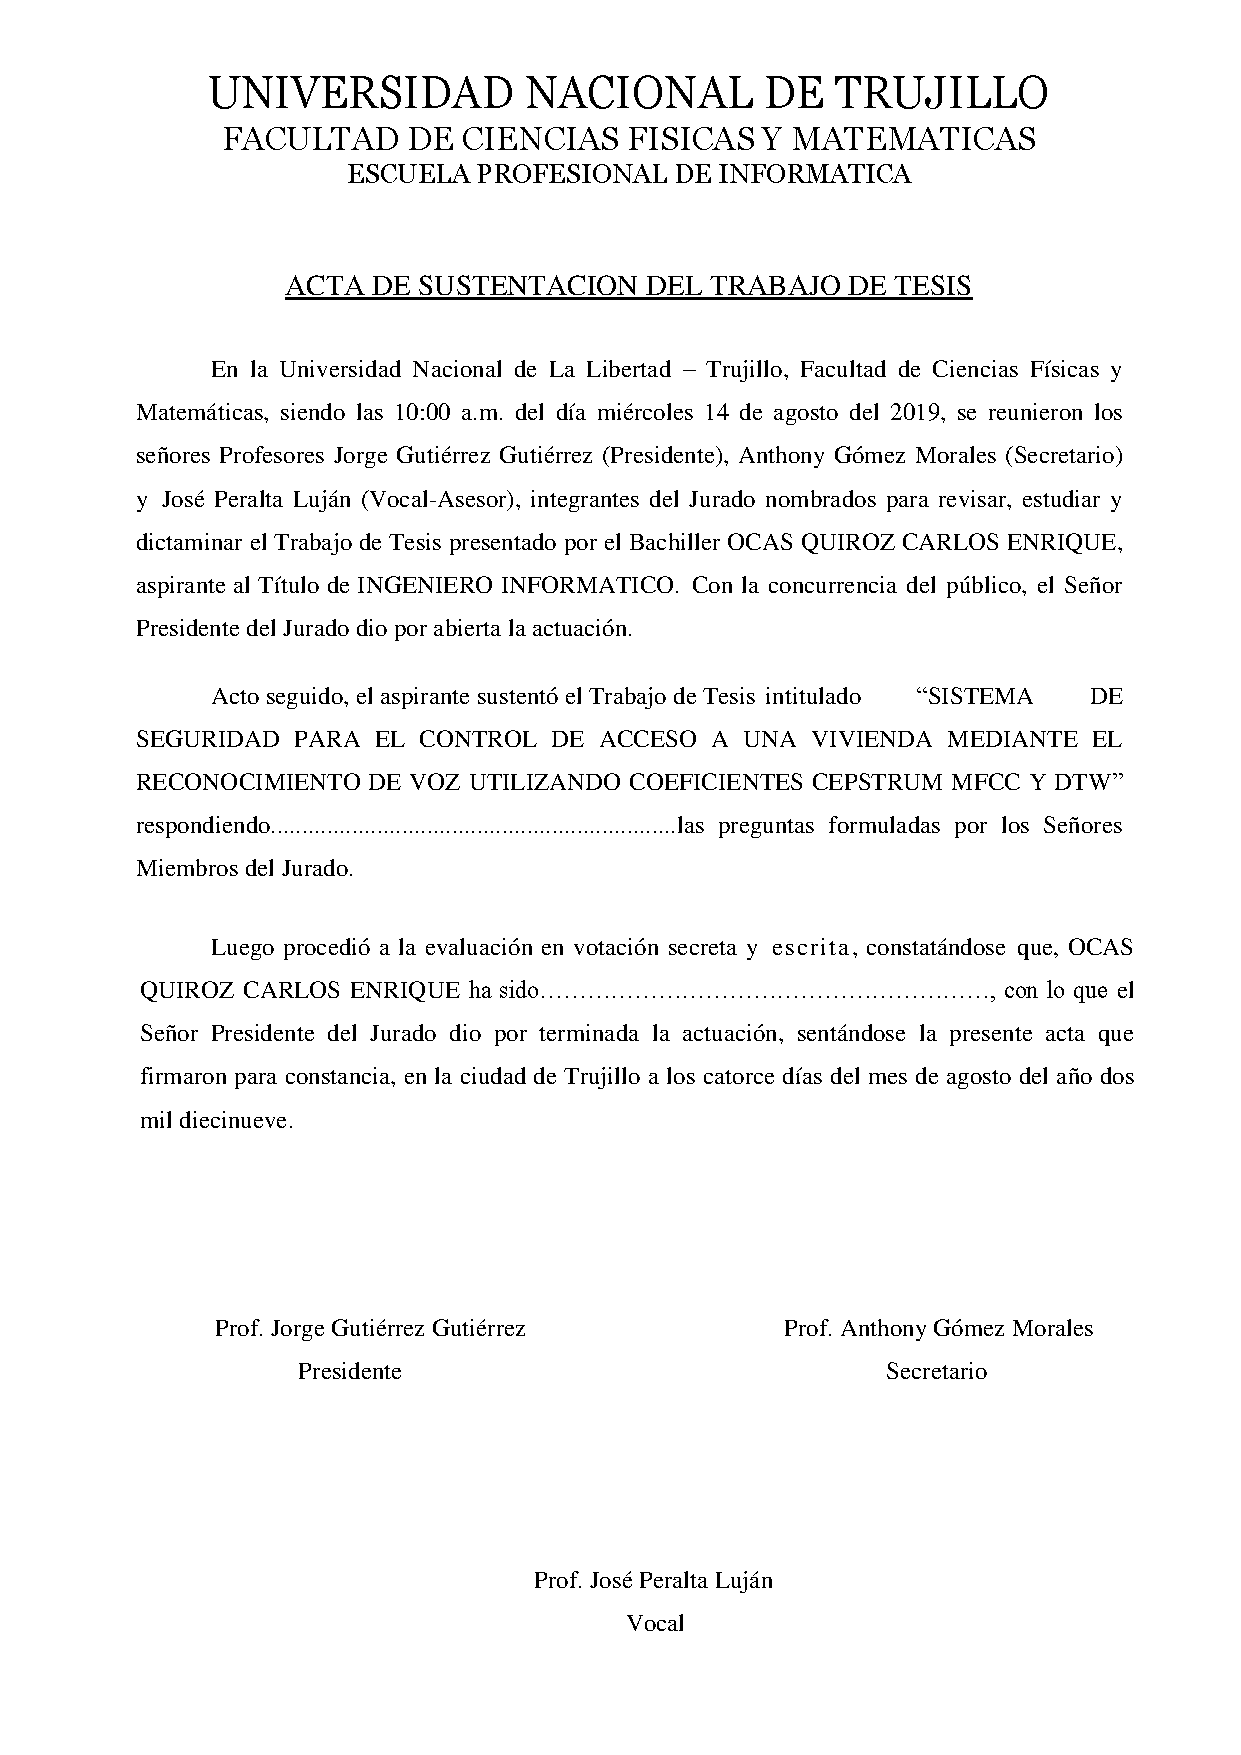
\includepdf[pages=-, offset=75 -75]{Documentos/ACTA_SUSTENTACION1.pdf}

%\setboolean{@twoside}{false}
%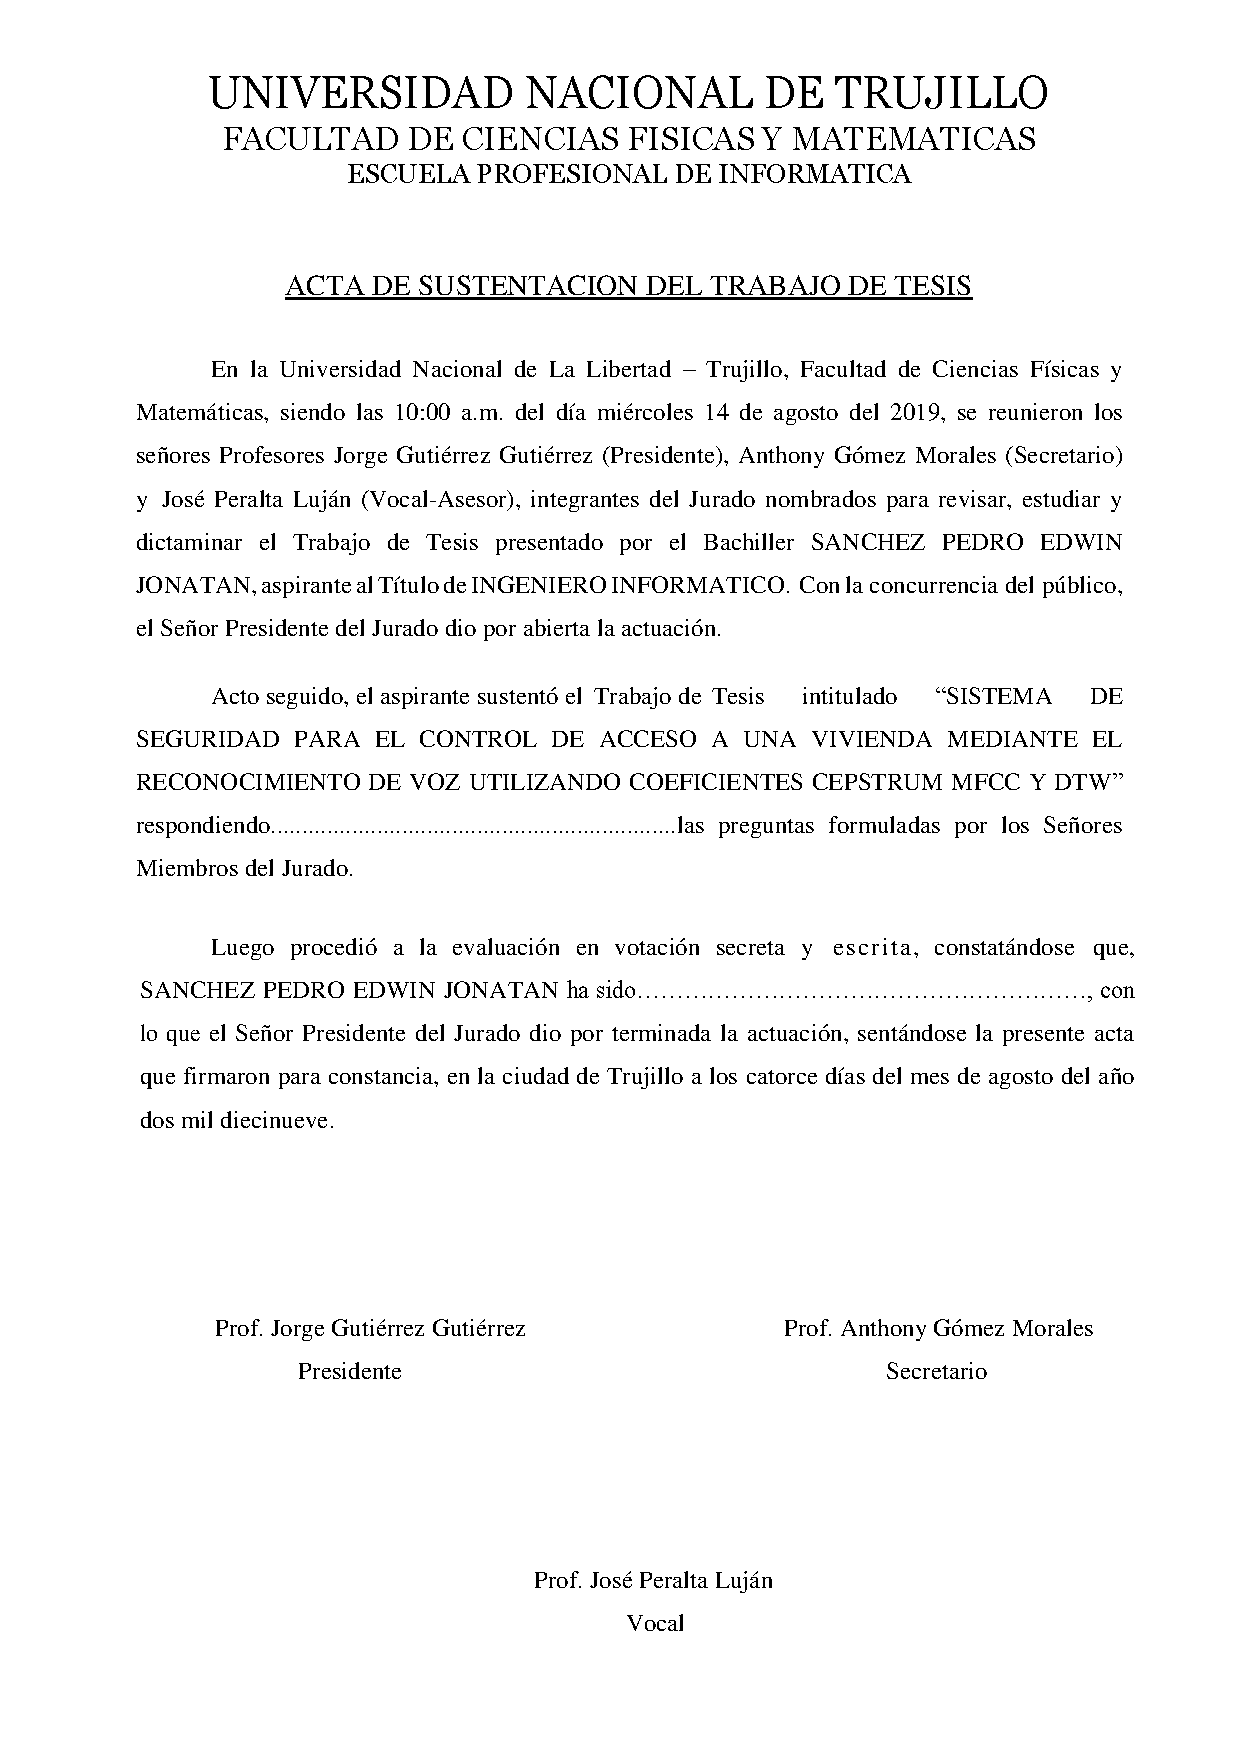
\includepdf[pages=-, offset=75 -75]{Documentos/ACTA_SUSTENTACION2.pdf}
%%%%%%%%%%%%%%%%%%%%%%%%%%%%%%%%%%%%%%%%%%%%%%%%%%%%%%%%%%%%%%%%%%%


%%%%%%%%%%%%%%%%%%%%%%%%%%%% RESUMEN%%%%%%%%%%%%%%%%%%%%%%
\newpage
\begin{center}
 \addcontentsline{toc}{chapter}{Resumen}
 {\bf\LARGE Resumen}
\end{center} 
\begin{quotation}
El presente trabajo busca desarrollar un sistema de seguridad para el control de acceso a una vivienda mediante el reconocimiento de voz del locutor dependiente del texto, donde el principal objetivo es identificar a cada miembro del hogar, quienes tendrán el acceso. El sistema permitirá que un usuario grabe una palabra clave a través del micrófono de un dispositivo móvil y este sea reconocido o no de la base de datos, permitiéndole o denegándole el acceso a la vivienda. El sistema estará conformado por 2 fases, la primera es la fase de extracción de características de la señal, para esto se usará una adaptación de los MFCC (Coeficientes Cepstrales en la Frecuencia de Mel) y la segunda fase es la del reconocimiento automático del locutor que estará basada en la técnica DTW (Alineamiento Temporal Dinámico), además de una lógica para la toma de decisióne para la identificación o no, o falsa identificación de un usuario. En relación a la configuración de los experimentos, los patrones de voz serán evaluados en 2 diferentes escenarios, uno con ruido y otro sin ruido. Para poder comprobar que el sistema sea confiable se harán 2 tipos de pruebas, una entre los usuarios del sistema tratando de acceder uno con el usuario del otro y otra donde personas ajenas a las almacenadas en la base de datos (usuarios no registrados) trataran de acceder.
\vskip 0.25cm
\hspace*{-0.6cm}{\bf Palabras claves:} Sistema de seguridad, control de acceso, reconocimiento de voz, reconocimiento del locutor, coeficientes cepstrales, alineamiento temporal dinámico.
\end{quotation}
%%%%%%%%%%%%%%%%%%%%%%%%%%%%%%%%%%%%%%%%%%%%%%%%%%%%%%%%%%%%%%%%%%%%%%%%%%%%%%%%%%%%


%%%%%%%%%%%%%%%%%%%%%%%%%%%%ABSTRACT%%%%%%%%%%%%%%%%%%%%%%
\newpage
\begin{center}
 \addcontentsline{toc}{chapter}{Abstract}
 {\bf\LARGE Abstract}
\end{center} 
\begin{quotation}
The present work seeks to develop a security system for the control of access to a home by means voice recognition of the speaker dependent on the text, where the main objective is to identify each member of the household, who will have access. The system will allow a user to record a keyword through the microphone of a mobile device and this is recognized or not from the database, allowing or denying access to the home. The system will consist of 2 phases, the first is the phase of extraction of characteristics of the signal, for this an adaptation of MFCC (Mel Frequency Cepstral Coefficients) will be used and the second phase is the automatic recognition of the speaker which will be based on the technique of DTW (Dynamic Time Warping), in addition to a logic for the decision making of the identification or not, or a false identification of a user. In relation to the configuration of the experiments, the speech patterns will be evaluated in 2 different scenarios, one with noise and the other without noise. In order to verify that the system is reliable, 2 types of tests will be done, one between the users of the home trying to access one with the user of the other and another where people other than those stored in the database (unregistered user) will try to access it. 
\vskip 0.25cm
\hspace*{-0.6cm}{\bf Keywords:} 
Security system, access control, voice recognition, speaker recognition, cepstral coefficients, dynamic time warping.
\end{quotation}
%%%%%%%%%%%%%%%%%%%%%%%%%%%%%%%%%%%%%%%%%%%%%%%%%%%%%%%%%%%%%%%%%%%%%%%%%%%%%%


%%%%%%%%%%%%%%%%%%%%%%%%%%% LISTA DE SIMBOLOS %%%%%%%%%%%%%%%%%%%%%%
\newpage
\addcontentsline{toc}{chapter}{Lista de símbolos}
 {\bf\LARGE Lista de símbolos}
 \vskip 1.5cm
Constantes: 
\begin{enumerate}
\item[(1)]$f_{s}$ \hspace*{0.9cm} Frecuencia de muestreo.
\item[(2)]$f_{max}$ \hspace*{0.45cm} Frecuencia máxima.
\item[(3)]$f_{min}$ \hspace*{0.5cm} Frecuencia mínima.
\item[(4)]$f_{N}$ \hspace*{0.8cm} Frecuencia de Nyquist.
\item[(5)]$T_{s}$ \hspace*{0.9cm} Periodo de muestreo.
\item[(6)]$\mu$ \hspace*{1.05cm} Tamaño de paso de adaptación del filtro adaptivo.
\item[(7)]$M$ \hspace*{0.85cm} Número de orden del filtro adaptivo.
\item[(8)]$\beta$ \hspace*{1.0cm} Constante de adaptación del filtro adaptivo.
\item[(9)]$c$ \hspace*{1.1cm} Constante de normalización del filtro adaptivo.
\item[(10)]$\alpha$ \hspace*{1.0cm} Valor del filtro preénfasis.
\item[(11)]$V$ \hspace*{1.0cm} Longitud de ventana en la segmentación.
\item[(12)]$S$ \hspace*{1.0cm} Valor de desplazamiento o solapamiento en la segmentación.
\item[(13)]$T$ \hspace*{0.9cm} Longitud de trama para la detección de inicio y fin de una palabra.
\item[(14)]$BC$ \hspace*{0.6cm} Número de bandas críticas del MFCC.
\item[(15)]$k_{l}$ \hspace*{0.9cm} Índice correspondiente a la frecuencia inferior.
\item[(16)]$k_{h}$ \hspace*{0.8cm} Índice correspondiente a la frecuencia superior.
\item[(17)]$P$ \hspace*{0.9cm} Slope constraint del DTW.
\item[(18)]$r$ \hspace*{1.0cm} Tamaño de ventana de ajuste del DTW.
\vskip 3cm
\end{enumerate} 
\vskip 0.3cm
Variables:
\begin{enumerate}
\item[(1)] $d(n) $ \hspace*{0.8cm} Señal de voz contaminada.
\item[(2)] $s(n)$ \hspace*{0.8cm} Señal de voz.
\item[(3)] $v_{0}(n)$ \hspace*{0.6cm} Señal de ruido en el micrófono primario.
\item[(4)] $v_{1}(n)$ \hspace*{0.6cm} Señal de ruido en el micrófono secundario.
\item[(5)] $w_{k}(n)$ \hspace*{0.5cm} Vector de pesos del filtro adaptivo.
\item[(6)] $e(n)$ \hspace*{0.8cm} Señal de error o respuesta deseada.
\item[(7)] $E_{n}$ \hspace*{1.0cm} Energía promedio por segmento.
\item[(8)] $E_{avg}$ \hspace*{0.75cm} Energía promedio de toda la señal.
\item[(9)] $M_{n}$ \hspace*{0.9cm} Magnitud promedio.
\item[(10)] $Z_{n}$ \hspace*{1.0cm} Cruce por ceros.
\item[(11)] $M_{sn}$ \hspace*{0.8cm} Magnitud del ruido.
\item[(12)] $Z_{sn}$ \hspace*{0.85cm} Cruce por ceros del ruido.
\item[(13)] $\mu_{Ms}$ \hspace*{0.75cm} Media de la magnitud del ruido.
\item[(14)] $\mu_{Zs}$ \hspace*{0.85cm} Media del cruce por ceros del ruido.
\item[(15)] $\sigma_{Ms}$ \hspace*{0.8cm} Desviación estándar de la magnitud del ruido.
\item[(16)] $\sigma_{Zs}$ \hspace*{0.9cm} Desviación estándar del cruce por ceros del ruido.
\item[(17)] $IZCT$ \hspace*{0.4cm} Umbral de cruce por ceros.
\item[(18)] $ITL$ \hspace*{0.7cm} Umbral de energía bajo.
\item[(19)] $ITU$ \hspace*{0.7cm} Umbral de energía alto.
\item[(20)] $IMX$ \hspace*{0.55cm} Energía máxima de la voz.
\item[(21)] $IMN$ \hspace*{0.7cm} Energía media del ruido de fondo.
\item[(22)] $x_{p}(n)$ \hspace*{0.8cm} Señal de voz con preénfasis.
\item[(23)] $x_{l}(n)$ \hspace*{0.85cm} Señal de voz segmentada.
\item[(24)] $x_{w}(n)$ \hspace*{0.75cm} Señal de voz ponderada.
\item[(25)] $w(n)$ \hspace*{0.9cm} Pesos de la ventana de Hamming.
\item[(26)] $N_{fft}$ \hspace*{1.0cm} Número de puntos de la transformada de Fourier.
\item[(27)] $X(k)$ \hspace*{0.9cm} Espectro en frecuencia de la transformada rápida de Fourier.
\item[(28)] $P(k)$ \hspace*{0.95cm} Espectro en potencia de la transformada rápida de Fourier.
\item[(29)] $\Delta f$ \hspace*{1.2cm} Resolución en frecuencia.
\item[(30)] $SF$ \hspace*{1.2cm} Separación en frecuencia.
\item[(31)] $N_{p}$ \hspace*{1.3cm} Número de puntos del espectro de potencia.
\item[(32)] $\Delta k$ \hspace*{1.2cm} Resolución por muestra del espectro.
\item[(33)] $P_{sc}$ \hspace*{1.2cm} Compresión del espectro en potencia.
\item[(34)] $C_{m}$ \hspace*{1.2cm} Transformada coseno discreta.
\item[(35)] $V_{mfcc}$ \hspace*{0.8cm} Coeficientes MFCC.
\item[(36)] $\Delta C_{k}$ \hspace*{0.8cm} Coeficientes MFCC delta.
\item[(37)] $\Delta \Delta C_{k}$ \hspace*{0.45cm} Coeficientes MFCC doble delta.
\item[(38)] $D_{T}$ \hspace*{1.05cm} Distancia total entre dos vectores.
\item[(39)] $D_{A}$ \hspace*{1.05cm} Distancia acumulada.
\item[(40)] $d$ \hspace*{1.35cm} Medida de distorsión.
\item[(41)] $z_{n}$ \hspace*{1.2cm} Patrón de referencia por la función de alineamiento.
\item[(42)] $U$ \hspace*{1.3cm} Umbral de decisión.
\item[(43)] $P(D)$ \hspace*{0.65cm} Distribución de probabilidad.
\item[(44)] $\mu^{intra}$ \hspace*{0.7cm} Media de las distancias intralocutor.
\item[(45)] $\mu^{inter}$ \hspace*{0.7cm} Media de las distancias interlocutor.
\item[(46)] $\sigma^{intra}$ \hspace*{0.7cm} Desviación estándar de las distancias intralocutor.
\item[(47)] $\sigma^{inter}$ \hspace*{0.7cm} Desviación estándar de las distancias interlocutor.
\end{enumerate}

